

% Gradient Info
  
\tikzset {_cb5yfaqw5/.code = {\pgfsetadditionalshadetransform{ \pgftransformshift{\pgfpoint{0 bp } { 0 bp }  }  \pgftransformscale{1 }  }}}
\pgfdeclareradialshading{_joeup2ykb}{\pgfpoint{0bp}{0bp}}{rgb(0bp)=(0,0,1);
rgb(0bp)=(0,0,1);
rgb(11.071428571428571bp)=(0,0,1);
rgb(18.21428571428571bp)=(0,0,1);
rgb(400bp)=(0,0,1)}
\tikzset{_imojnisr0/.code = {\pgfsetadditionalshadetransform{\pgftransformshift{\pgfpoint{0 bp } { 0 bp }  }  \pgftransformscale{1 } }}}
\pgfdeclareradialshading{_rtyi7lnb6} { \pgfpoint{0bp} {0bp}} {color(0bp)=(transparent!29);
color(0bp)=(transparent!29);
color(11.071428571428571bp)=(transparent!74);
color(18.21428571428571bp)=(transparent!99);
color(400bp)=(transparent!99)} 
\pgfdeclarefading{_8yyx6lp0v}{\tikz \fill[shading=_rtyi7lnb6,_imojnisr0] (0,0) rectangle (50bp,50bp); } 

% Gradient Info
  
\tikzset {_k0um4nwr3/.code = {\pgfsetadditionalshadetransform{ \pgftransformshift{\pgfpoint{0 bp } { 0 bp }  }  \pgftransformscale{1 }  }}}
\pgfdeclareradialshading{_t5f54e7qb}{\pgfpoint{0bp}{0bp}}{rgb(0bp)=(1,0,0);
rgb(0bp)=(1,0,0);
rgb(11.071428571428571bp)=(1,0,0);
rgb(18.21428571428571bp)=(0,0,1);
rgb(400bp)=(0,0,1)}
\tikzset{_tzlzpm80e/.code = {\pgfsetadditionalshadetransform{\pgftransformshift{\pgfpoint{0 bp } { 0 bp }  }  \pgftransformscale{1 } }}}
\pgfdeclareradialshading{_1t6g4v21q} { \pgfpoint{0bp} {0bp}} {color(0bp)=(transparent!29);
color(0bp)=(transparent!29);
color(11.071428571428571bp)=(transparent!75);
color(18.21428571428571bp)=(transparent!99);
color(400bp)=(transparent!99)} 
\pgfdeclarefading{_s4yeh3kfb}{\tikz \fill[shading=_1t6g4v21q,_tzlzpm80e] (0,0) rectangle (50bp,50bp); } 

% Gradient Info
  
\tikzset {_kpiqgjc5j/.code = {\pgfsetadditionalshadetransform{ \pgftransformshift{\pgfpoint{0 bp } { 0 bp }  }  \pgftransformscale{1 }  }}}
\pgfdeclareradialshading{_t2ces11zz}{\pgfpoint{0bp}{0bp}}{rgb(0bp)=(0,1,0);
rgb(0bp)=(0,1,0);
rgb(11.071428571428571bp)=(0,1,0);
rgb(18.21428571428571bp)=(0,0,1);
rgb(400bp)=(0,0,1)}
\tikzset{_g6v3ksomg/.code = {\pgfsetadditionalshadetransform{\pgftransformshift{\pgfpoint{0 bp } { 0 bp }  }  \pgftransformscale{1 } }}}
\pgfdeclareradialshading{_6ktb8xhs1} { \pgfpoint{0bp} {0bp}} {color(0bp)=(transparent!29);
color(0bp)=(transparent!29);
color(11.071428571428571bp)=(transparent!75);
color(18.21428571428571bp)=(transparent!99);
color(400bp)=(transparent!99)} 
\pgfdeclarefading{_o76gac6ql}{\tikz \fill[shading=_6ktb8xhs1,_g6v3ksomg] (0,0) rectangle (50bp,50bp); } 
\tikzset{every picture/.style={line width=0.75pt}} %set default line width to 0.75pt        

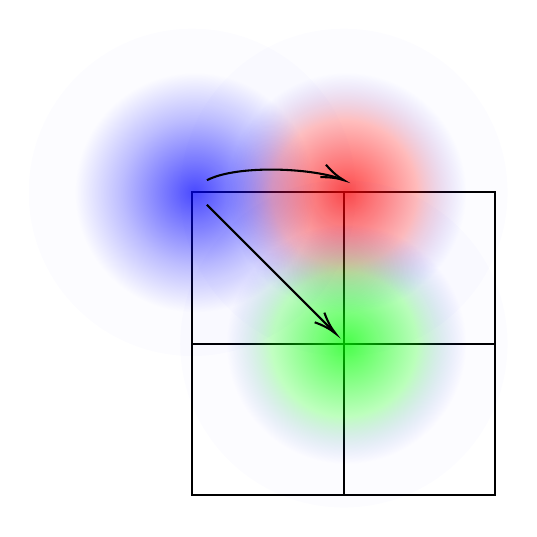
\begin{tikzpicture}[x=0.75pt,y=0.75pt,yscale=-1,xscale=1]
%uncomment if require: \path (0,346); %set diagram left start at 0, and has height of 346

%Shape: Grid [id:dp8110941042559912] 
\draw  [draw opacity=0] (167,85) -- (313,85) -- (313,231) -- (167,231) -- cycle ; \draw   (240,85) -- (240,231) ; \draw   (167,158) -- (313,158) ; \draw   (167,85) -- (313,85) -- (313,231) -- (167,231) -- cycle ;
%Shape: Circle [id:dp47180655307663555] 
\draw  [draw opacity=0][shading=_joeup2ykb,_cb5yfaqw5,path fading= _8yyx6lp0v ,fading transform={xshift=2}] (88.15,85) .. controls (88.15,41.45) and (123.45,6.15) .. (167,6.15) .. controls (210.55,6.15) and (245.85,41.45) .. (245.85,85) .. controls (245.85,128.55) and (210.55,163.85) .. (167,163.85) .. controls (123.45,163.85) and (88.15,128.55) .. (88.15,85) -- cycle ;
%Shape: Circle [id:dp046329586169280956] 
\draw  [draw opacity=0][shading=_t5f54e7qb,_k0um4nwr3,path fading= _s4yeh3kfb ,fading transform={xshift=2}] (161.15,85) .. controls (161.15,41.45) and (196.45,6.15) .. (240,6.15) .. controls (283.55,6.15) and (318.85,41.45) .. (318.85,85) .. controls (318.85,128.55) and (283.55,163.85) .. (240,163.85) .. controls (196.45,163.85) and (161.15,128.55) .. (161.15,85) -- cycle ;
%Curve Lines [id:da20408642695880563] 
\draw    (174,79.15) .. controls (188.4,71.65) and (224,73.19) .. (238.32,78.47) ;
\draw [shift={(240,79.15)}, rotate = 204.12] [color={rgb, 255:red, 0; green, 0; blue, 0 }  ][line width=0.75]    (10.93,-3.29) .. controls (6.95,-1.4) and (3.31,-0.3) .. (0,0) .. controls (3.31,0.3) and (6.95,1.4) .. (10.93,3.29)   ;
%Shape: Circle [id:dp5914644578546182] 
\draw  [draw opacity=0][shading=_t2ces11zz,_kpiqgjc5j,path fading= _o76gac6ql ,fading transform={xshift=2}] (161.15,158) .. controls (161.15,114.45) and (196.45,79.15) .. (240,79.15) .. controls (283.55,79.15) and (318.85,114.45) .. (318.85,158) .. controls (318.85,201.55) and (283.55,236.85) .. (240,236.85) .. controls (196.45,236.85) and (161.15,201.55) .. (161.15,158) -- cycle ;
%Straight Lines [id:da9442638680984972] 
\draw    (174,91) -- (234.59,151.59) ;
\draw [shift={(236,153)}, rotate = 225] [color={rgb, 255:red, 0; green, 0; blue, 0 }  ][line width=0.75]    (10.93,-3.29) .. controls (6.95,-1.4) and (3.31,-0.3) .. (0,0) .. controls (3.31,0.3) and (6.95,1.4) .. (10.93,3.29)   ;




\end{tikzpicture}
